% ****** Start of file aipsamp.tex ******
%
%   This file is part of the AIP files in the AIP distribution for REVTeX 4.
%   Version 4.2a of REVTeX, December 2014
%
%   Copyright (c) 2014 American Institute of Physics.
%
%   See the AIP README file for restrictions and more information.
%
% TeX'ing this file requires that you have AMS-LaTeX 2.0 installed
% as well as the rest of the prerequisites for REVTeX 4.2
%
% It also requires running BibTeX. The commands are as follows:
%
%  1)  latex  aipsamp
%  2)  bibtex aipsamp
%  3)  latex  aipsamp
%  4)  latex  aipsamp
%
% Use this file as a source of example code for your aip document.
% Use the file aiptemplate.tex as a template for your document.
\documentclass[%
 aps,
 jmp,%
 amsmath,amssymb,
%preprint,%
 reprint,%
%author-year,%
%author-numerical,%
]{revtex4-2}

\usepackage{enumitem}
\usepackage{braket}

\usepackage{graphicx}% Include figure files
\usepackage{dcolumn}% Align table columns on decimal point
\usepackage{bm}% bold math
\usepackage{mathtools}
\usepackage{amsthm,amssymb, hyperref}
\usepackage{xcolor}
%\usepackage[mathlines]{lineno}% Enable numbering of text and display math
%\linenumbers\relax % Commence numbering lines
\DeclarePairedDelimiter{\ceil}{\lceil}{\rceil}

\begin{document}

\preprint{AIP/123-QED}

\title[Quantum Accelerated Causal Tomography...]{Quantum Accelerated Causal Tomography: \\Circuit Considerations For Applications In Bioinformatics and AGI}% Force line breaks with \\

% \title[Quantum Accelerated Causal Tomography...]{Quantum Accelerated Causal Tomography: \\Circuit Considerations Towards Applications}% Force line breaks with \\

\thanks{All authors contributed equally to this work.}

\author{Tamal Acharya}
\email{tamal\_974@yahoo.com}
\affiliation{QWorld Association.}
\affiliation{Purdue University, West Lafayette, USA.} 
%
\author{Akash Kundu}
\email{akundu@iitis.pl}
\thanks{corresponding author}
\affiliation{QWorld Association.}

\affiliation{Institute of Theoretical and Applied Informatics, Polish Academy of Sciences,}
\affiliation{Joint Doctoral School, Silesian University of Technology, Gliwice, Poland}

%
\author{Aritra Sarkar}
\email{a.sarkar-3@tudelft.nl}
\affiliation{QWorld Association.}
\affiliation{Quantum Machine Learning group, QuTech, \\
	Delft University of Technology, Delft, The Netherlands}%

\date{\today}% It is always \today, today,
             %  but any date may be explicitly specified
             

\begin{abstract}
In this work, we study quantum computing algorithms for accelerating causal inference. Specifically, we extend the formulation of causal hypothesis testing presented in [\textit{Nat Commun} 10, 1472 (2019)] for practical scenarios. Through an implementable algorithm, we show that the error probability introduced in the previous work requires modification. The practical scenario which is followed by a theoretical description is constructed as a scalable quantum gate-based algorithm on IBM Qiskit. We present the circuit construction of the oracle embedding the causal hypothesis and assess the associated gate complexities. Additionally, our demonstration on a simulator platform validate the predicted speedup. We discuss applications of this framework for causal inference use cases in bioinformatics and artificial general intelligence.
\end{abstract}

\keywords{causal inference, causal hypothesis, error probability, process distance}%Use showkeys class option if keyword
                              %display desired
\maketitle

\iffalse
\begin{quotation}
The ``lead paragraph'' is encapsulated with the \LaTeX\ 
\verb+quotation+ environment and is formatted as a single paragraph before the first section heading. 
(The \verb+quotation+ environment reverts to its usual meaning after the first sectioning command.) 
Note that numbered references are allowed in the lead paragraph.
%
The lead paragraph will only be found in an article being prepared for the journal \textit{Chaos}.
\end{quotation}
\fi

\section{\label{s1}Introduction}


Despite the huge success of machine learning~(ML) algorithms based on deep neural networks, these systems are inscrutable black-box models.
This hampers users' trust in the system and obfuscated the discovery of algorithmic biases arising from flawed generated processes that are prejudicial to certain inputs (e.g. racial discrimination).
Explainable artificial intelligence~(XAI) focuses on human understanding of the decision from the learned solution, as white-box models.
These models provide results that are understandable for domain experts, thus providing transparency, interpretability, and explainability.
XAI algorithms provide a basis for justifying decisions, tracking and thereby verifying them, improving the algorithms, and exploring new facts.
There has been relatively slow progress in XAI, despite realizing its importance as we increasingly automate critical systems.
Early advances in XAI were based on symbolic reasoning systems and truth maintenance systems.
To achieve causal reasoning, rule-based learning and logic-based inference systems were proposed.
Methods to address inherent opaque modern methods like deep learning-based neural networks and genetic algorithms include layer-wise relevance propagation and local interpretability.
There exist other ML algorithms (e.g. decision trees, Bayesian classifiers, additive models) that generate interpretable models i.e. the model components (e.g., the weight of a feature, a path in a decision tree, or a specific rule) can be directly inspected to understand the predictions.
However, these models are not general and scalable to compete with the adoption and impact of neural networks.
On the other hand, symbolic reasoning systems were abandoned owing to the difficulty in scaling these systems for a large number of parameters.

The capability of \textit{quantum computation allows us to scale symbolic reasoning models by encoding the classical rules as a superposition of quantum states or processes}~\cite{sarkar2021estimating}.
Thus, quantum mechanics provide enhanced ways to identify causal links.
Certain quantum correlations can be used to infer classical causal relationships~\cite{ried2015quantum,fitzsimons2015quantum}.
This could overcome the apprehension of existing classical approaches being pursued in XAI.

In this article, we will explore how we can distinguish quantum processes by their causal structure.
Specifically, we study the construction proposed in \cite{chiribella2019quantum} towards a quantum circuit implementation on the IBM Qiskit quantum programming language.
In doing so, we uncover: (i) the implementation aspects of the causal oracle, (ii) the gate and qubit complexity of the full algorithm, and (iii) the dependence of the error probability on the set of processes/hypothesis being tested.
While the current technology readiness level of quantum systems prevents us from demonstrating this causal reasoning within a broader application framework, we present the quantum kernel that can be readily embedded within a software pipeline for applications in bioinformatics and artificial general intelligence~(AGI).
In particular, it will be useful in XAI pipelines~\cite{lavin2021simulation,maruyama2021categorical}.

The remaining article is organized as follows. 
In {Section~[\ref{sec:overview-causal-inference}]} we briefly review the specifics of causal reasoning and some of the well-studied techniques. 
A discussion on the basic concepts and quantum advantage of causal hypothesis testing is given in {Section~[\ref{sec:causal-hypothesis-testing}]}. 
In the following {Section~[\ref{sec:prob-formulation}]} we describe the problem formulation; containing the main findings of the article. 
Here we define a model implementation on Qiskit followed by a correction factor introduced in the error probability based on our empirical results; which we call \textit{practical error probability}. 
Finally, in {Section~[\ref{sec:application framework}]} we discuss some potential use cases in bioinformatics and artificial general intelligence.
The corresponding quantum resources of gates and qubits are assessed for realistic cases.
{Section~[\ref{sec:conclusion}]} concludes the article.
\section{\label{sec:overview-causal-inference}Overview of causal inference}
% Identifying cause–effect relations is an essential tool in science.
% Simulation Intelligence: Towards a New Generation of Scientific Methods
% % https://arxiv.org/abs/2112.03235
% This is generally accomplished through classical statistical trials where alternative hypotheses are tested against each other.
% \subsection{Overview of causal inference}
Causal inference refers to an intellectual discipline that considers the assumptions, study designs, and estimation strategies that allow researchers to draw conclusions on the cause-effect relationships between data. 
% The term `causal conclusion' used here refers to a conclusion regarding the effect of a causal variable (often referred to as the ‘treatment’ under a broad conception of the word) on some outcome(s) of interest. 
The dominant perspective on causal inference in statistics has philosophical underpinnings that rely on the consideration of counterfactual states. 
In particular, it considers the outcomes that could manifest given exposure to each of a set of treatment conditions (dynamics of a specific causal variable). 
Causal effects are defined as comparisons between these potential outcomes. 
Causal inference consists of a family of statistical methods whose purpose is to answer the question of why something happens. 
Standard approaches in statistics, such as regression analysis, are concerned with quantifying how changes between two variables are associated, with no directional sense. 
In contrast to that, causal inference methods are used to determine whether changes in a variable X cause changes in another variable Y or vice-versa. 
% Therefore, unlike methods that are concerned with associations only, causal inference approaches can answer the question of why Y changes. 
If X is causally related to Y, then Y's change can (at least partially) be explained in terms of X's change.

% \subsection{Problems with causal inference}
\subsection{Challenges of performing causal inference}

% In this section we discuss the problems with causal inferences and some of the limitations of state-of-the-art causal models.

Causal models are based on the idea of potential outcomes. 
The fundamental problem for causal inference is that, for any individual unit (a physical object at a particular point in time), we can observe only one of the potential outcomes, either Y(1) (under treatment) or Y(0) (under no treatment). 
As we observe the value of the potential outcome under only one of the possible treatments~\footnote{A treatment is an action that can be applied or withheld from that unit.}, namely, the treatment actually assigned, hence the potential outcome under the other treatment is missing.

The inadequacy of the causal models is due to their failure to include relevant spatial and structural information in a way that does not render the model non-explanatory, unmanageable, or inconsistent with the basic assumptions of causal graph theory. 
Making valid causal inferences is challenging because it requires high-quality data and adequate statistical methods. 
One prominent example of common non-causal methodology is the erroneous assumption of correlative properties as causal properties. 
Correlated phenomena may not carry inherent causation. 
Regression models are designed to measure variance within data relative to a theoretical model. 
This suggests that there is nothing in the data that presents high levels of covariance that have any meaningful relationship among them. 
This suggests the absence of a proposed causal mechanism with predictive properties or a random assignment of treatment. 
The presupposition that two correlated phenomena are inherently related is a logical fallacy, known as spurious correlation.
\begin{itemize}[noitemsep,nolistsep]
\item \textbf{Causation does not imply association}
	For example, we want to compare the impact of an academic degree on the income of a middle-aged individual. 
	The person might have attended the academic degree or might not have. 
	To calculate the causal effect of having an academic degree, we need to compare the output in both situations, which is not possible. 
	This dilemma is a fundamental problem of causal inference. 
	The challenge in causal inference is that \textit{all potential outcomes are not observed}, we only observe one.
	Another example is described by the situation of -- a black cat ran under the fence and I tripped and fell over. 
	We could have tripped anyway. 
	It had nothing to do with the cause of the cat running under the fence, i.e., \textit{associated events do not imply causal connection}.
	
    \item \textbf{Correlation does not prove causality}
	
	Causal inference is usually a missing data problem~\cite{guo2020survey} and we tend to make \textit{assumptions to make up for the missing causes/variables}. 
	An example is a correlation between people eating ice cream and people drownings. 
	It could indicate that eating ice cream affects drowning. 
	The actual correlation is between the season (summer) and these otherwise unrelated things. 
	In this case, the missing cause is the season. 
	Another example is the correlation between higher SAT scores and a greater number of books in the house of the student taking the tests. 
	Causal inference would imply that the number of books directly affects the SAT scores, when in reality, they are both affected by something else (in this case most likely a higher average intelligence in the household). 
	Causal inference is the process of drawing a conclusion about a causal connection based on the occurrence of an effect.
\end{itemize}
The main difference between causal inference and inference of association is that the former analyzes the response of the effect variable when the cause is changed, and in the latter, inferences about the strength of association between variables are made using a random multivariate sample of data drawn from the population of interest.
Thus, in causal inference, we have access to the additional information about the variable/s on which the intervention has occurred between two sets of associated data samples.
Another problem of causal inference is that the cause and the effect may have occurred by chance rather than by intention.

The causal effect of a drug on systolic blood pressure, one month after the drug dosage vs no exposure to the drug dosage can be represented as a comparison of systolic blood pressure that would be measured at the time of given exposure to the drug with the systolic blood pressure that would be measured at the same point in time in the absence of exposure to the drug.
The challenge for causal inference is that we are not generally able to observe both of these states: at some point in time when we are measuring the outcomes, each individual either has had drug exposure or has not.
From the data perspective, there are some open problems to review regarding the great potential of learning causality with data. 
Such as the study of heterogeneous groups, learning causality with imbalanced data, and learning causality with complex variables.
\subsection{Classical techniques in causal inference}
Causal inference is conducted via the study of systems where the measure of one variable is suspected to affect the measure of another. 
Causal inference is conducted with regard to the scientific method. 
The first step of causal inference is to formulate a falsifiable null hypothesis, which is subsequently tested with statistical methods.
Frequentist statistical inference uses statistical methods to determine the probability that the data occur under the null hypothesis by chance.
Bayesian inference is used to determine the effect of an independent variable.

Common frameworks for causal inference include the causal pie model (component-cause)~\cite{rothman2005causation}, Pearl's structural causal model (causal diagram and do-calculus)~\cite{pearl2000models}, structural equation modeling, and Rubin's causal model (potential-outcome)~\cite{imbens2015causal}.

The most frequently used causal models can be grouped into two kinds: causal Bayesian networks and structural equation models (which are distinct but closely related). %, cf. Spirtes 2010
Causal graph models combine mathematics and philosophy: the mathematical elements are Directed Acyclic Graphs (DAGs) and probability theory (with focus on conditional independence); the philosophical elements are assumptions about the relationship between causation and probability~\cite{spirtes2000causation}.

\subsection{Algorithmic machine learning}

An alternative approach to causal inference based on algorithmic generative models is currently gaining popularity. 
\cite{zenil2019causal} describes the process of performing causal deconvolution using this technique.
This paper talks about the different generating mechanisms by which complex data is produced. 
The authors introduced a universal, unsupervised, and parameter-free model-oriented approach based upon algorithmic probability that decomposes an observation into its most likely algorithmic generative sources. 
It uses causal calculus to infer model representations. 
% This novel framework is being evaluated by using the ability of the methods to separate data from observations that are being produced by discrete dynamical systems such as cellular automata and complex networks.
This research suggests that cellular automata offer an optimal testbed as they are discrete dynamical systems that are able to illustrate an algorithm's inner workings because of their visual nature. 
% They can be interpreted as 1-D objects that produce 2-D images when adding runtime and producing highly integrated 2-D objects whose rows are strongly and causally connected and are thus ideal testing cases.

The approach is similar to the Data Generating Process~(DGP) in statistics which posits that each set of observations is just a snapshot that we see and is just one instance of the many that could have been possible. 
This approach also tells us that each and every data point is being generated from a data-generating process which can be taken as coming from some distribution of data and is just a sample of the total population. 
We try to understand the DGP while analyzing that data and try to find out what could have been the sources that generated those data.
The research introduces algorithmic probability and the coding theorem. 
The deconvolution algorithm breaks a dataset into groups that do not share certain features, i.e. essentially causal clustering and algorithmic partition by probable generative mechanism.
These methods are conceptually different from traditional clustering and partition in machine learning approaches.

% Usually we have a parameter to maximize but 
Ultimately the purpose of this method is to distinguish components that are generated similarly from those that are generated differently. 
In information theoretic terms, the question the method answers is, what are the elements (e.g. nodes or edges) that can break a network into the components that maximize their algorithmic information content, i.e., those elements that preserve the information about the underlying programs generating the data.
% This is similar to the Max-Cut algorithm which also works on a similar way. 
It basically preserves maximum information while removing redundant components. 
% We also have to make sure that while removing the components we should not be removing those components which if they are removed reduces the total information of the system or graph.
% The authors also mentions the time complexities of the order of O(M2) and O(M) based on the algorithms used. 
This new conceptual framework involves parameter-free methods to tackle the problem of information decomposition by means of causal deconvolution based on the fundamental theory of algorithmic probability which defines optimal inductive inference.

\begin{figure*}[t!]
	\centering %LBRT
	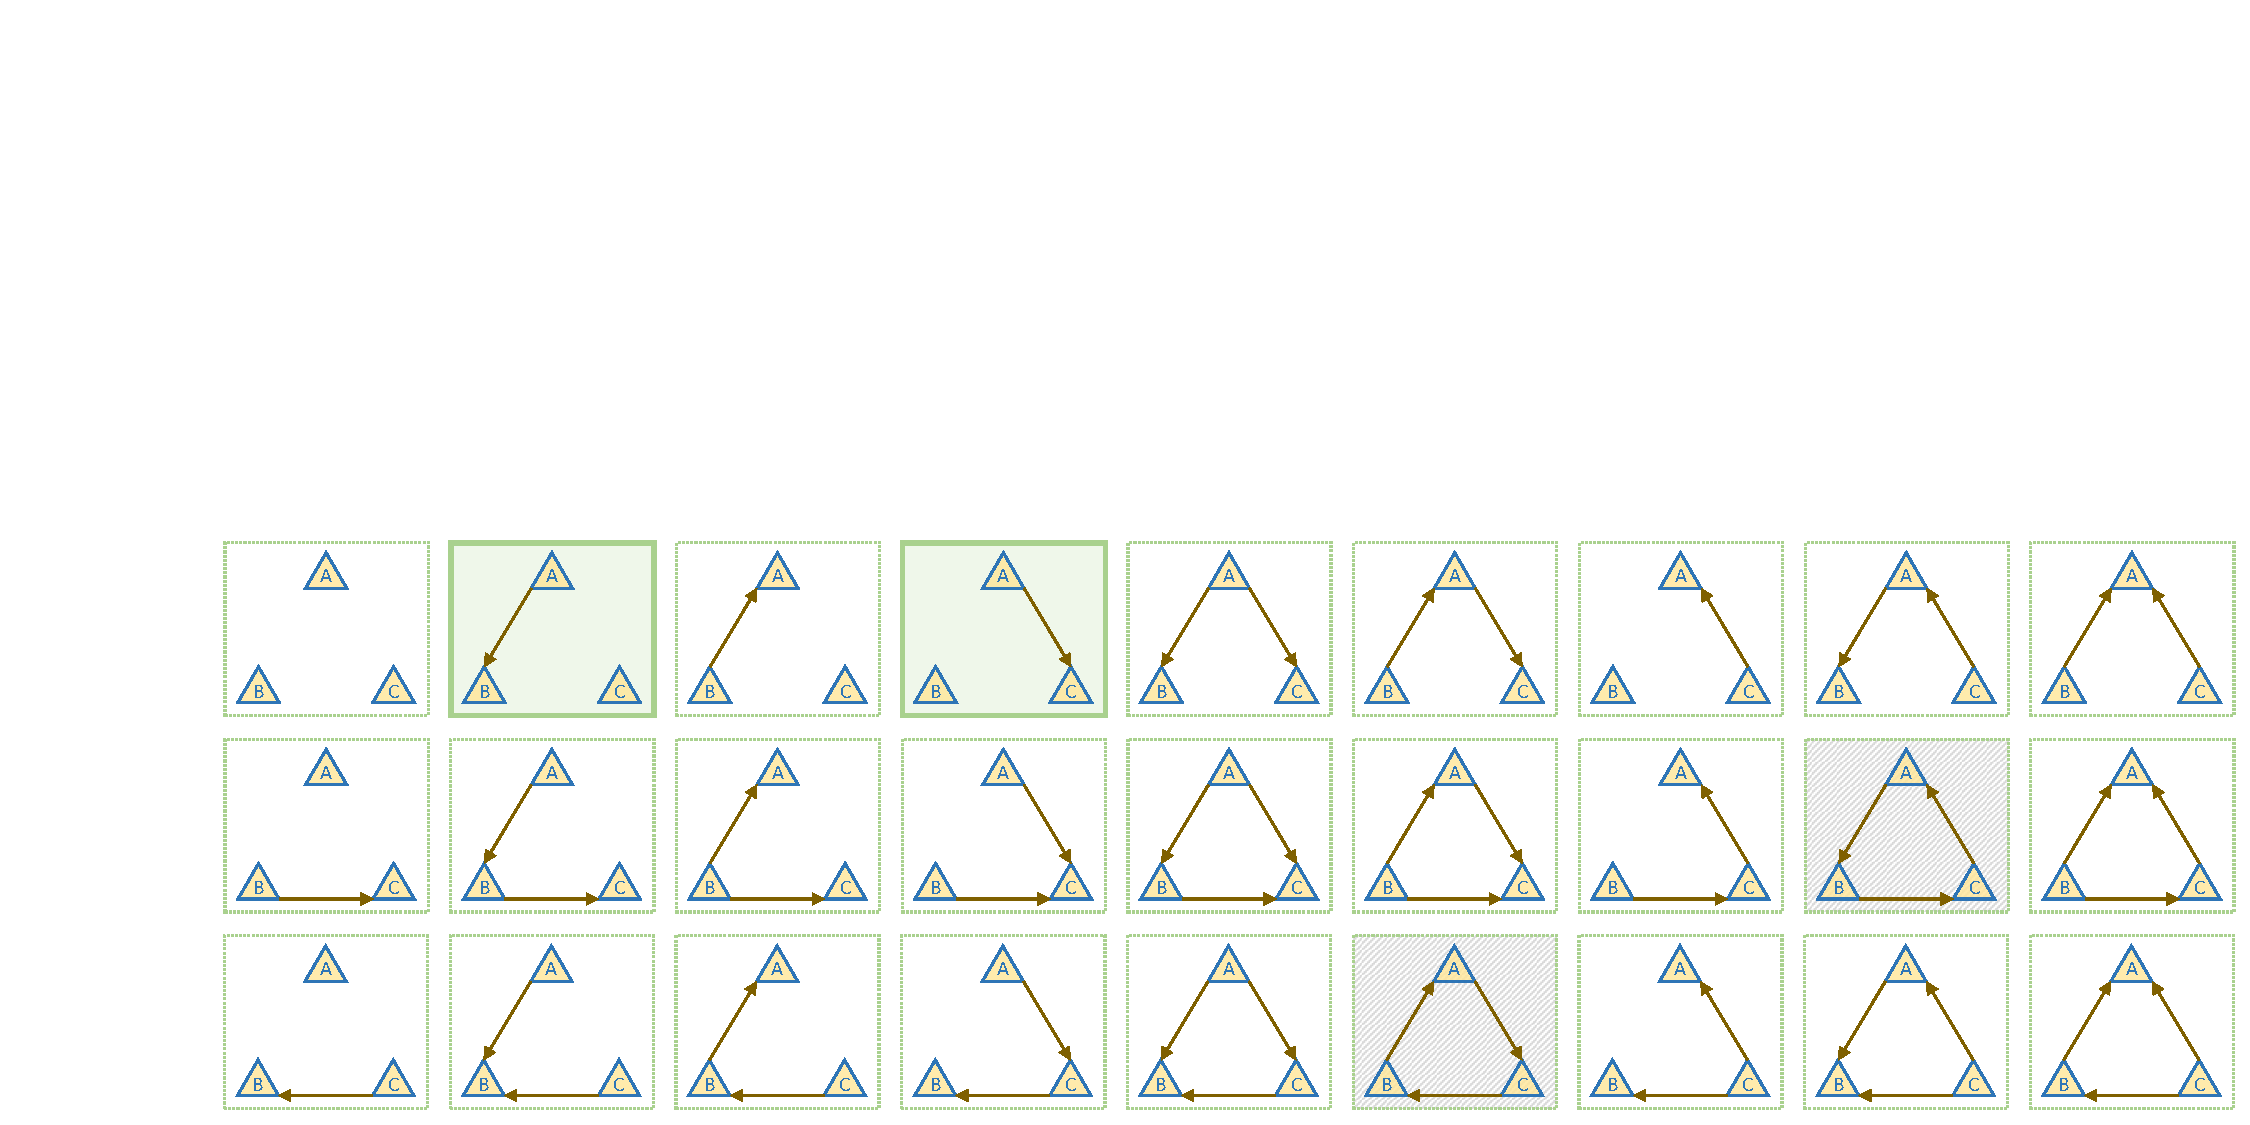
\includegraphics[clip, trim=3cm 0cm 0cm 9cm,width=\textwidth]{3vci.pdf}
	\caption{All possible causal relations for 3 variables. Blocks shaded grey have causal loops (and are typically not considered). The set of blocks shaded green indicates a case of causal hypothesis testing.}
	\label{fig:3vci}
\end{figure*}

\subsection{Quantum computation and algorithmic information}

The synergy between quantum computation and algorithmic information has been studied extensively in \cite{sarkar2022applications}.
Two main directions were explored, that can be applied for causal inference.

In \cite{sarkar2021estimating} a global/objective view is presented, which involves quantum automata for algorithmic information.
A framework for causal inference based on algorithmic generative models is developed. 
This technique of quantum-accelerated experimental algorithmic information theory~(QEAIT) can be ubiquitously applied to diverse domains. 
Specifically for genome analysis, the problem of identifying bit strings capable of self-replication is presented. 
A new quantum circuit design of a quantum parallel universal linear bounded automata~(QPULBA) model is developed that enables a superposition of classical models/programs to be executed, and their properties can be explored. 
The automaton prepares the universal distribution as a quantum superposition state which can be queried to estimate algorithmic properties of the causal model.

In \cite{sarkar2021qksa} a local/subjective view is presented, which involves universal reinforcement learning in quantum environments.
This theoretical framework can be applied to automated scientific modelling. 
A universal artificial general intelligence formalism is presented that can model quantum processes. 
The developed quantum knowledge-seeking agent~(QKSA) is an evolutionary general reinforcement learning model for recursive self-improvement. 
It uses resource-bounded algorithmic complexity of quantum process tomography~(QPT) algorithms. 
The cost function determining the optimal strategy is implemented as a mutating gene within a quine. 
The utility function for an individual agent is based on a selected quantum distance measure between the predicted and perceived environment.

These techniques motivate our research in this article.
Unlike quantum/classical data-driven machine learning, these primitives of QEAIT and QKSA preserve the explanatory power of the model the learning converges to by exploring the space of programs on an automata model.
The QPULBA model (in QEAIT) and QPT algorithms (in QKSA) can be generalized to a causal oracle and causal tomography respectively.

\section{Causal hypothesis testing} \label{sec:causal-hypothesis-testing}

A canonical approach in causal inference is to formulate different hypotheses on the cause–effect relations and test them against each other.
This technique is typically used when there is some knowledge of the characteristic of the phenomenon that is being tested.
The complete search space of directed graphs between events grows exponentially.
An exhaustive example of 3 variable causal relations is shown in Fig.~[\ref{fig:3vci}].
In causal hypothesis testing~(CHT) a subset of these graphs is considered as the set of hypotheses being tested against each other.
For example, in Fig.~[\ref{fig:3vci}], we can consider, two hypotheses (shaded in green):
\begin{itemize}[nolistsep,noitemsep]
	\item A causes B, C is independent
	\item A causes C, B is independent.
\end{itemize}

\subsection{Quantum advantage in classical causal hypothesis testing}
%----------------
\begin{figure*}[t!]
	\centering
	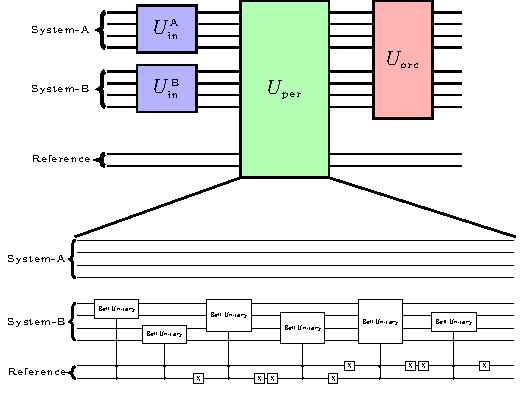
\includegraphics[width = 0.7\linewidth]{bortoni.pdf}
	\caption{The illustration of the model implementation. Where we also show the decomposition of $U_\textrm{per}$ for $ N_\textrm{A} = N_\textrm{B} = 4$.}
	\label{fig:perm-circuit}
\end{figure*}
%----------------
Quantum information enables a richer spectrum of causal relations that is not possible to access via classical statistics.
Most research in this direction is towards exploring causality in the quantum context~\cite{costa2016quantum,giarmatzi2019quantum,javidian2021quantum,bai2021quantum,bai2020efficient,bavaresco2021strict}.
Our focus in this work is specifically using the quantum formulation to provide a \textit{computational advantage with respect to a classical technique on classical data}.

This problem is studied extensively in \cite{chiribella2019quantum}.
The research analyzes the task of identifying the effect of a given input variable.
The constructed quantum strategy reduces the error probability by an exponential amount, doubling the decay rate of the error probability with the number of accesses to the relevant variables. 
This decay rate is the highest achievable rate allowed by quantum mechanics, even if one allows for exotic setups where the order of operations is indefinite.
The key ingredient of the quantum speedup is the ability to run multiple equivalent experiments in a quantum superposition.
This can be used for the detection of a causal link between two variables, and in the identification of the cause of a given variable, as well.

The set of allowed causal relationships depends on the physical theory, which determines which maps can be implemented by physical processes.
In classical physics, cause-effect relations are typically represented by conditional probability distributions, while, in quantum theory, they are described by quantum channels, i.e., completely positive trace-preserving maps transforming density matrices of system A into density matrices of system B.
\section{Problem formulation} \label{sec:prob-formulation}
Contrary to the general case considered in~\cite{chiribella2019quantum}, our formulation is towards an implementable quantum circuit that is demonstrated on the Qiskit \texttt{statevector} simulator. 
This formulation is detailed here. 

The input variables (causes) are denoted by the set $C = \{c_0, c_1,\dots, c_{|C|-1}\}$, while the output variables (effects) are denoted by the set $E = \{e_0, e_1,\dots, e_{|E|-1}\}$.
If we consider an equal number of input and output variables to implement a quantum circuit to preserve unitarity, i.e., $|C| = |E| = k$. 
We maintain the simplification in \cite{chiribella2019quantum} that all variables are of equal length, 
\begin{equation}
d = |c_i| = |e_j|,
\end{equation}
where $c_i \in C$ and $e_j \in E$.
Thus, each variable has $2^d$ states. 
Furthermore, we consider that each effect is a permutation of only one cause, i.e. the map from $C$ to $E$ is a bijective function, one-to-one correspondence, or invertible function.
\subsection{Model implementation}
In our implementation, we consider a general case where the access to interventions on the causes and the effects are not equal.
As a proof-of-concept, we implement a causal hypothesis testing with control over $1$ cause $C=\{c_0\}$ and measurement capability over $2$ potential effects $E = \{e_0,e_1\}$.
These hypotheses are mutually exclusive, i.e., 
\begin{itemize}
    \item Hypothesis 0: $e_0 \leftarrow U c_0$, $e_1$ is independent of $c_0$
    \item Hypothesis 1: $e_1 \leftarrow U c_0$, $e_0$ is independent of $c_0$
\end{itemize}
where $U$ is a unitary map between the cause and effect.
    
To design a quantum circuit, all variables that are potentially inspected as causes need to be assigned a quantum information placeholder.
The total such placeholders required are, 
\begin{equation}
k = \max\{|C|,|E|\}.
\end{equation}
For this example, $k=2$ sets of qubit registers are used, namely system A and system B, both initialized to the all-zero state.
The initialization and interaction between these two systems and how it affects the performance of causal tomography are studied.

The practical implementation is decomposed into the following steps:

\begin{itemize}
    
    \item The number of times the causal process (oracle) is queried is denoted by $N$. 
    The larger the $N$, the lesser the error probability. 
    For the simulations, the value is chosen as $N = N_A = N_B = 4$.
    
    \item $U_\textrm{in}^\textrm{A}$, $U_\textrm{in}^\textrm{B}$, represents the initialization of the system A and B respectively. 
    The causes are thus, $c_0 = U_\textrm{in}^\textrm{A} \ket{0}^{\otimes d}$ and $c_1 = U_\textrm{in}^\textrm{B} \ket{0}^{\otimes d}$. 
    These are used to study the circuit for various cases of initialization.
    For the simulations, the variable length $d=1$. 
    For each set of $d$ qubits among the $N$ copies, the same unitary needs to be applied. 

    \item $U_\textrm{per}$, decomposes into parallel strategies which represent the possible ways to group inputs into entangled pairs.
 % abcdef
 % ab cd ef
 % ab ce df
 % ab cf de
 % ac bd ef
 % ac be df
 % ac bf de
 % ad bc ef
 % ad be cf
 % ad bf ce
 % ae bc df
 % ae bd cf
 % ae bf dc
 % af bc de
 % af bd ce
 % af be cd
 % 6*5/2 = 15
% $4! / 2!*2^2 = 4.3/4 = 3$
% $6! / 3!*2^3 = 6.5.4/8 = 15$
For $n$-qubits, the total possible such linearly independent pair combinations are $r = \dfrac{n!}{(n/2)! \times 2^{n/2}}$, where,
\begin{equation}
    n = N\times|C|\times d
\end{equation}
Since we have control over only $1$ cause, $n = 4\times1\times1 = 4$, and $r = 4!/(2!\times2^2) = 3$.
The number of qubits in the reference to encode these states are $N_{\textrm{ref}} = \lceil\log_2 r \rceil$. In our case, $N_{\textrm{ref}} = \lceil \log_2 3 \rceil = 2$

    \item $U_\textrm{orc}$, represents an unknown process that induces a causal relation between inputs and outputs.
    For example, for the two hypotheses considered, it can be an \texttt{Identity} gate for hypothesis 0 and a \texttt{Swap} gate for hypothesis 1.
\end{itemize}
The qubit requirement of this model grows as:
\begin{equation}
N \times k \times d + \ceil{\log_2 \left( \dfrac{n!}{\frac{n}{2}! \times 2^{\frac{n}{2}}} \right)}
\label{eq:qubit-requirement}
\end{equation}

The model is illustrated through an implementable quantum circuit in Fig.~[\ref{fig:perm-circuit}] in Appendix.
\begin{figure*}[tbh!]
	\centering
	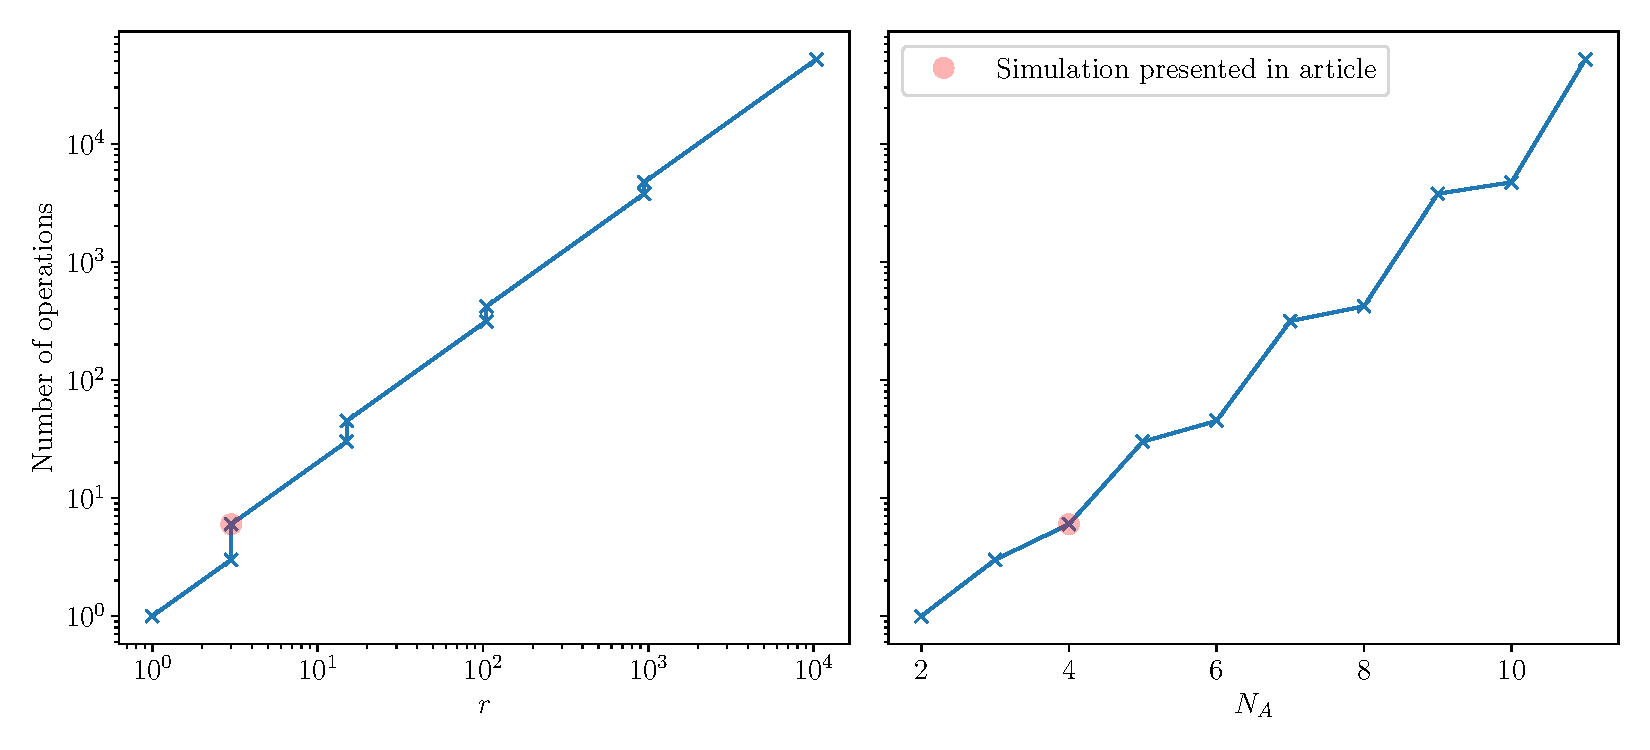
\includegraphics[width = 0.9\linewidth]{number_of_operations.pdf}
	\caption{Illustration of the number of controlled Bell unitary required to implement the $U_\textrm{per}$ in respect to a number of linearly independent state $r$ (left-hand side figure) and with the dimension of the subsystem (right-hand side figure).}
	\label{fig:permutation-resource}
\end{figure*}
In the previous work, one of the innovations introduced was to entangle the inputs for the parallel strategy instead of initializing with a tensor product state which reduces the exponential measurement resource requirement by correlating the basis. But the cost of implementing the entangled initialization was not analyzed. 

Through our model implementation, we are able to show that the operations required to implement the $U_\textrm{per}$ grows faster than exponentially with the dimension of the subsystem as illustrated in Fig.~[\ref{fig:permutation-resource}] but linear in respect to the linearly independent states i.e. $r$.



\subsection{Practical error probability}

While the number of controllable causes $|C|$ and the encoding length of the causes $d$ depends on the problem formulation, the number of queries, i.e. $N$ and thereby $r$ is a free parameter.
It can be chosen based on the available quantum circuit resources of the number of qubits in the quantum processor, the decoherence time, and gate error probability, such that the pragmatic error remains low.

In the quantum case, the coherent superposition of equivalent configuration gives the error probability \cite{chiribella2019quantum}
\begin{equation}
p_\textrm{err} = \frac{r}{2d^N}\left( 1-\sqrt{1-r^{-2}} \right) \xrightarrow[]{r>>1}\frac{1}{4rd^N},\label{eq:limiting-case-equation}
\end{equation}
where $r$ is the number of linearly independent states.
It is suggested that the Eq.\eqref{eq:limiting-case-equation} gives the limiting case error probability. 

However, in a more general case, the error probability of causal hypothesis testing should be dependent on the two specific hypotheses.

As an example, if the unitary oracles implementing the two causal hypotheses, $U_\textrm{orc}^{H0} = U_\textrm{orc}^{H1}$, then $p_\textrm{err} =1$.

To incorporate this dependence on the relative distinguishability of the hypotheses, we introduce a correction factor proportional to the process distance between the two oracles. 
Hence the modified Eq.\eqref{eq:limiting-case-equation} takes the form
\begin{widetext}
\begin{equation}
p_\textrm{err}^\textrm{prac} = \frac{r}{2d^N}\left( 1-\sqrt{1-r^{-2}} \right)\Delta\left[U_\textrm{orc}^{H0}, U_\textrm{orc}^{H1}\right] \xrightarrow[]{r>>1}\frac{\Delta\left[U_\textrm{orc}^{H0}, U_\textrm{orc}^{H1}\right]}{4rd^N},\label{eq:practical-case-equation}
\end{equation}
\end{widetext}

There are many choices for the distance $\Delta$ function between the hypotheses and need to be chosen based on the experimental and theoretical specifications of the application. 
For this investigation, we have considered three distance measures
\begin{enumerate}[nolistsep,noitemsep]
	\item \textit{Trace distance} which is defined by 
	\begin{equation}
	\Delta = \frac{1}{2}\textrm{Tr}\left(\rho_\textrm{orc}-\rho_\textrm{orc}^\textrm{alter}\right),
	\end{equation}
	where $\rho$ represents the Choi representation of the unitary.
	\item \textit{Bures distance} which defined as 
	\begin{equation}
	\Delta = 2\left(1-\sqrt{F(\rho_\textrm{orc},\rho_\textrm{orc}^\textrm{alter})}\right),
	\end{equation}
	where $F$ quantifies the process fidelity between the Choi representation of oracles.
	\item \textit{Hilbert-Schmidt distance} which is defined by
\begin{equation}
	\Delta = \textrm{Tr}\left[\left(\rho_\textrm{orc} - \rho_\textrm{orc}^\textrm{alter}\right)^2\right].
\end{equation}
\end{enumerate}

\newpage
\subsection{Numerical results}

To obtain numerical results we consider the setup represented in Fig.~[\ref{fig:perm-circuit}] where the dimension of the subsystems are the same.
IBM's open-source quantum computer simulator \texttt{qiskit} was used to simulate the above-mentioned implementation.
Throughout the numerical investigation, we choose the oracle unitary as follows:

\begin{widetext}
\begin{equation}
U_\textrm{orc}^{H_{0/1}}(\theta_x,\theta_y) = 
\big[\textrm{CSWAP}(c,A_i,B_i)^{\otimes N}\big]
\big[\textrm{RX}(c,\theta_x)\otimes\mathbb{I}(A_i)^{\otimes N}\otimes \textrm{RY}(B_i,\theta_y)^{\otimes N}\big]
\label{eq:oracles}
\end{equation}
\end{widetext}
\begin{figure*}[tbh!]
	\centering
	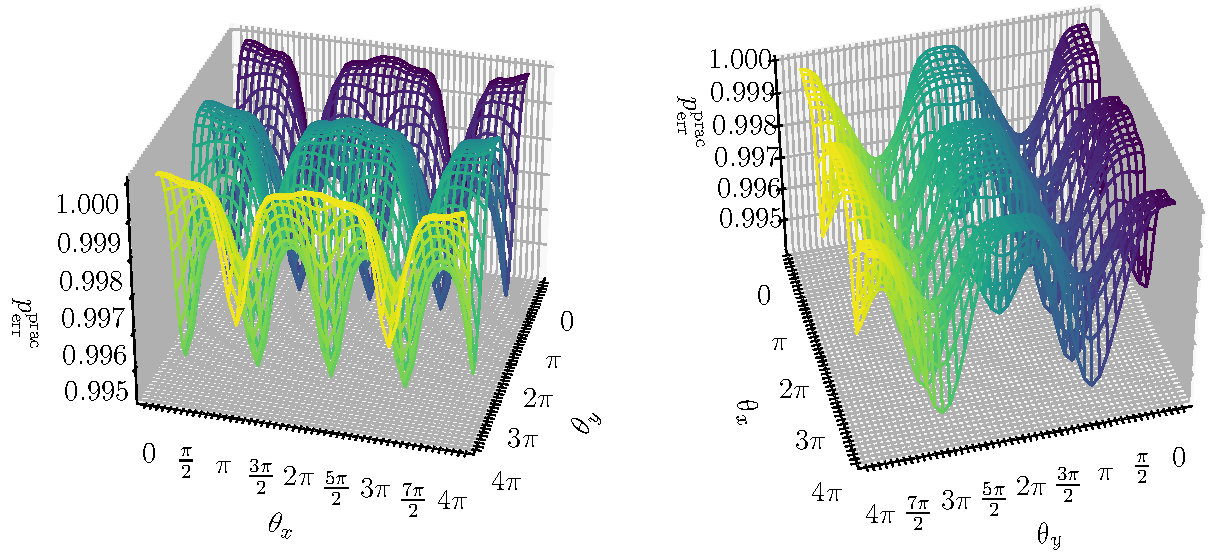
\includegraphics[width = \linewidth]{practical_case_error_prob-crop.pdf}
	\caption{On the left-hand side we illustrate the variety of practical case error probability with respect to $\theta_x$. On the right-hand side we show the variation of practical case error probability with respect to oracle angle $\theta_y$.}
	\label{fig:practical-case-error-plot}
\end{figure*}

The parameter $\theta_x$ allows interpolating between the two hypotheses discussed before.
To obtain the specific hypothesis cases of \texttt{Identity} and \texttt{SWAP}, the above parameters are set to $U_\textrm{orc}^{H_{0}}(0,0)$ and $U_\textrm{orc}^{H_{1}}(\pi,0)$ respectively.
The dependence of the error probability of distinguishing two hypotheses with respect to the relative difference is enquired by varying the alternate hypothesis to
\begin{equation}
U_\textrm{orc}^{H_{0/1}} = 
\begin{cases}
U_\textrm{orc}^{H_{0}}(0,0), \\\\
U_\textrm{orc}^{H_{1}}(\theta_x,0)
\end{cases}
\label{eq:alternate-hypothesis-theta-x}
\end{equation}



The result is illustrated in Fig.[\ref{fig:prac_prob_with_thetas}] and left-hand side of Fig.[\ref{fig:practical-case-error-plot}].
It can be identified that the lowest error (or most distinguishability) is achieved for the Identity vs. SWAP case, when the angle is an odd multiple of $\pi$, (i.e., the RX gate is a Pauli-X) while for even multiples of $\pi$, the hypotheses are not distinguishable, with an error probability of 1.

In the following demonstration, we test the dependence of the error probability on arbitrary unitaries applied to a specific hypothesis when they were originally maximally distinguishable.
For this, we set the parameters to
\begin{equation}
U_\textrm{orc}^{H_{0/1}} = 
\begin{cases}
U_\textrm{orc}^{H_{0}}(0,0), \\\\
U_\textrm{orc}^{H_{1}}(\pi,\theta_y)
\end{cases}
\label{eq:alternate-hypothesis-theta-y}
\end{equation}
The result is shown in Fig.[\ref{fig:prac_prob_with_thetas}] and right-hand side of Fig.[\ref{fig:practical-case-error-plot}].
It is seen that the error probability is independent of local operations on a specific hypothesis.

% $U_\textrm{orc} = \mathbb{I}^{\otimes N_\textrm{A}}\otimes \mathbb{I}^{\otimes N_\textrm{B}}$ and as for the alternate hypothesis we choose

% \begin{equation}
% U_\textrm{orc}^\textrm{alter}(\theta)= 
% \begin{cases}
% \lvert0\rangle^{\otimes N_\textrm{A}} \otimes \mathbb{I}^{\otimes N_\textrm{B}}, \\\\
% \lvert1\rangle^{\otimes N_\textrm{A}} \otimes \textrm{RY}(\theta)^{\otimes N_\textrm{B}}.
% \end{cases}
% \label{eq:alternate-hypothesis}
% \end{equation}

% We have utilized IBM open-source quantum computer simulator \texttt{qiskit} and simulated the above-mentioned implementation.
% The total qubits for $N_\textrm{A}=N_\textrm{B}=N=4$ 

% qubits using \texttt{statevector\_simulator}.

% The main motivation behind the choice of \texttt{CRY$(\theta)$} as the alternate hypothesis is by varying the parameter $\theta$ one can go from a non-correlated to a fully correlated state.
%----------------

In the Fig.~[\ref{fig:prac_prob_with_thetas}] for setting of oracle \eqref{eq:alternate-hypothesis-theta-x} we observe that the error probability varies as
\[
p_\textrm{err}^\textrm{prac} = 
\begin{cases}
p_\textrm{err}^\textrm{max}\;\;\;\;\;\;\;\;\;\;\;\;\;\;\;\;\;\;\;\;\;\;\;\;\;\;\;\;\; \textrm{for}\;\; \theta = (2m+1)\pi/2,\\

p_\textrm{err}^\textrm{min} \;\;\;\;\;\;\;\;\;\;\;\;\;\;\;\;\;\;\;\;\;\;\;\;\;\;\;\;\; \textrm{for}\;\; \theta = m\pi,\\

p_\textrm{err}^\textrm{min}<p_\textrm{err}^\textrm{prac} <p_\textrm{err}^\textrm{max}\;\;\;\;\; \textrm{otherwise},
\end{cases}
\]

and in the Fig.~[\ref{fig:prac_prob_with_thetas}] for setting of oracle \eqref{eq:alternate-hypothesis-theta-y} we observe that the error probability varies as
\[
p_\textrm{err}^\textrm{prac} = 
\begin{cases}
p_\textrm{err}^\textrm{max}\;\;\;\;\;\;\;\;\;\;\;\;\;\;\;\;\;\;\;\;\;\;\;\;\;\;\;\;\; \textrm{for}\;\; \theta = 2m\pi,\\

p_\textrm{err}^\textrm{min} \;\;\;\;\;\;\;\;\;\;\;\;\;\;\;\;\;\;\;\;\;\;\;\;\;\;\;\;\; \textrm{for}\;\; \theta = (2m+1)\pi,\\

p_\textrm{err}^\textrm{min}<p_\textrm{err}^\textrm{prac} <p_\textrm{err}^\textrm{max}\;\;\;\;\; \textrm{otherwise},
\end{cases}
\]
where $m=0,1,2,\ldots$.
Through the numerical simulation we show that the $p_\textrm{err}^\textrm{max} = 1.0$, when two hypothesis coincide i.e. $\theta_x = 0$, $\theta_y = 0$; and $p_\textrm{err}^\textrm{min} = 0.994$, when we consider the alternate hypothesis $\theta_x = \pi$, $\theta_y = 0$.
%----------
\begin{figure}[t!]
	\centering
	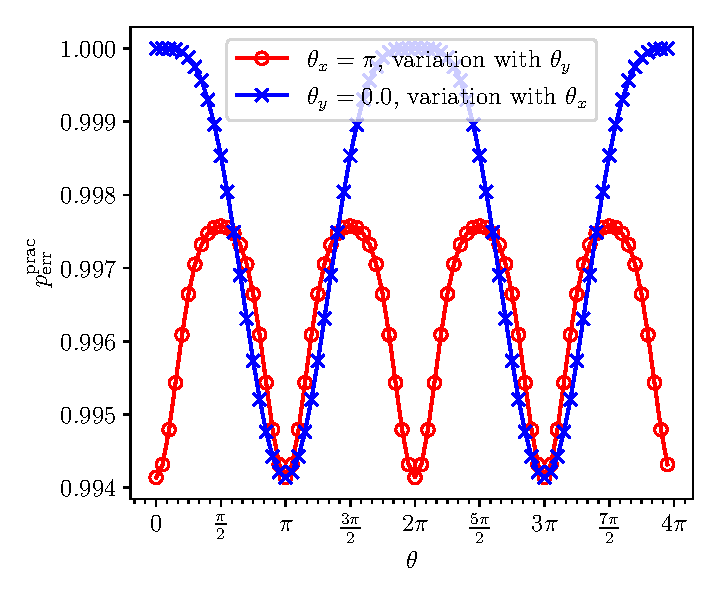
\includegraphics[width = 1.0\linewidth]{prac_prob_vs_thetas.pdf}
    \caption{Illustration of variation of practical case error probability with respect to $\theta_x$, when $\theta_y = 0.0$ (blue line)  and $\theta_y$, when $\theta_x = \pi$ (red line).}
	\label{fig:prac_prob_with_thetas}
\end{figure}

\begin{figure}[t!]
	\centering
	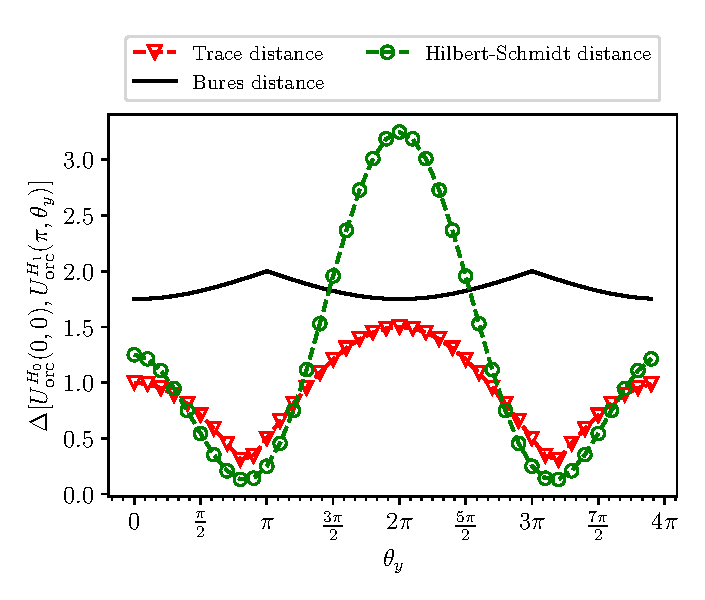
\includegraphics[width = 1.0\linewidth]{diff_process_dist.pdf}
	\caption{Illustration variation of different distance measure with respect to the oracle angle $\theta_y$.}
	\label{fig:diff_dist_meas}
\end{figure}
%----------
It should be noted that the construction we used for numerical simulation has the following parameter values: $r=3$, $d=2$ and $N=4$. In this setting, the limiting case probability that is given in ref.\cite{chiribella2019quantum} and expressed in Eq.\eqref{eq:limiting-case-equation} is constant at
\begin{equation}
p_\textrm{err} = 0.00536.
\end{equation}
We observe that the results for the limiting case and the numerically simulated error probability are distinct. This is because the $p_\textrm{err}$ was introduced purely theoretically where the authors evaluated it for a maximally mixed alternate hypothesis. In a practical case (numerical simulation of the quantum circuit) it is not feasible to construct a maximally mixed oracle. This leads us to introduce the realistic case error probability. In the practical scenario (see oracle presented in \eqref{eq:oracles}) the alternate hypothesis is implementable in currently widely available hardware and through the simulation, we show that the limiting case error probability in the practical scenario requires a slight modification. This modification is reflected through the introduction of the distance between the oracles under consideration i.e. $\Delta\left[U_\textrm{orc}^\textrm{alter},U_\textrm{orc}\right]$. Based on this in Eq.\eqref{eq:practical-case-equation} we introduce a modified version of limiting case error probability that can be evaluated realistically on quantum hardware.

Next, it is logical to examine the variation of process distance with respect to the oracle parameter $\theta_y$. In Fig.~[\ref{fig:diff_dist_meas}] we illustrate the distance between the null hypothesis $U_\textrm{orc}^{H_{0}}(0,0)$ and the alternate hypothesis $U_\textrm{orc}^{H_{1}}(\pi,\theta_y)$ for a class of distance measure. 

For the sake of the demonstration, we present the observation for \textit{Trace distance}, \textit{Bures distance} and the \textit{Hilbert-Schmidt distance}. It can be seen that the characteristics of \textit{Trace} and \textit{Hilbert-Schmidt} are similar, due to the fact that both of them fundamentally depends on the difference in the Choi representation of the oracles, whereas \textit{Bures distance} depends on the process distance.
% The numerical illustration suggests

\section{Application framework} \label{sec:application framework}

With the quantum kernel presented above, in this section, we will develop an application framework in the context and discuss two consequential applications.

\subsection{Bioinformatics}

Applications of causal inference are widespread in bioinformatics.
Specifically, inferring a causal network of the variables is practised in medical diagnostics and genomics.

For example, causal discovery in Alzheimer’s pathophysiology is studied in ref.~\cite{shen2020challenges} with 9 variables (13 with longitudinal data).
Similarly, for detecting causal regulatory interactions between genes, tools like \texttt{Scribe-py}~\cite{qiu2020inferring} are currently used.
Exemplary use cases of (i) transcription expression dynamics hierarchy of C. elegans' early embryogenesis and (ii) core regulatory network responsible for myelopoiesis are used for this research, with the latter graph consisting of 10 nodes.

The current generation of quantum processors supports 100s of qubits and is expected to scale to 1000s in a few years.
However, the challenge is the limitation of the decoherence time and gate errors, which bounds the runtime of the algorithm that can be effectively executed.
For a causal graph in the order of 10 causes/effects, a causal specificity bits of $d=1$ and with $N=100$, the estimation presented in Eq.\eqref{eq:qubit-requirement} is $6262$ qubits.
Keeping in mind the potential of near-term devices, pragmatic industrial cases of causal tomography will remain outside the reach of quantum computing in the near term.

% how to make the oracle? grover search?

\subsection{Artificial General Intelligence}

In the long term, quantum accelerated causal inference will be beneficial for artificial general intelligence.
Quantum accelerated AGI is still in its infancy. In ref.~\cite{catt2020gentle}, the authors proposed the AIXI-q reinforcement learning agent empowered with quantum counting. Meanwhile, ref.~\cite{sarkar2021estimating} proposed an exhaustive enumeration of all causal oracles (or, alternatively, all bounded-size programs of a Turing machine).
These techniques can develop synergies with the quantum accelerated causal tomography circuit as developed in this article.

In theoretical physics, automated science tools, specifically in the context of causal set theory, will also find the causal tomography framework of crucial use. 

\section{Conclusion} \label{sec:conclusion}

In this article, we extend the previously introduced~\cite{chiribella2019quantum} causal hypothesis testing formulation for the practical scenario. This lead us to develop a scalable quantum gate-based algorithm which can be implemented in the available near-term quantum devices. Through the algorithm formulation, we empirically show that the limiting case error probability that is represented in ref.~\cite{chiribella2019quantum} requires modification. In our work, this modification is done by introducing process distance between the causal hypotheses, to the formulation of error probability. We term this modified version of error probability as \textit{practical case error probability} which is stricter than the limiting case. Additionally, our implementation enables an estimation of the pragmatic gate complexity of the causal tomography entangled pair indexing.

Furthermore, the proposed algorithm is implemented using the open-source quantum programming and simulation platform \texttt{qiskit}. As in ref.~\cite{chiribella2019quantum} it is shown that the quantum advantage holds for generalized probabilistic theory so the practical case that we present here is optimal in any scenario.

Our motivation for this project is driven by the increasing focus on causal inference in machine learning.
Besides monitoring the information flow in future quantum communication networks, as discussed in ref.\cite{chiribella2019quantum}, causal tomography is crucial for understanding the bounds of general intelligence and for bioinformatics use cases.
In our future work, we aim to apply our developed quantum accelerated causal tomography framework for these applications.

\begin{acknowledgments}
This project was initiated under the QIntern 2021 project ``Reinforcement Learning Agent for Quantum Foundations".
Therefore we would like to thank the organizers of the program and QWorld Association. 
We would also like to thank QIndia for providing us with a collaboration platform for the ideas motivating this research.
AK was partially supported by the Polish National Science Center (NCN) under the grant agreement $2019/33/B/ST6/02011$.
\end{acknowledgments}

\appendix

% \section{Circuit Implementation}
% Here we provide an illustration of the circuit that has been implemented to obtain the numerical results. Th dimension of the subsystem is kept at $4$ due to the hardware limitations.

% \section{Poster}
% Here attach the poster which has been presented in the \texttt{Causalworlds: The interface between quantum and relativistic causality, foundations and practicalities}. The link to the conference  \href{https://causalworlds.ethz.ch/}{https://causalworlds.ethz.ch/}.
%\begin{figure*}
%\centering
%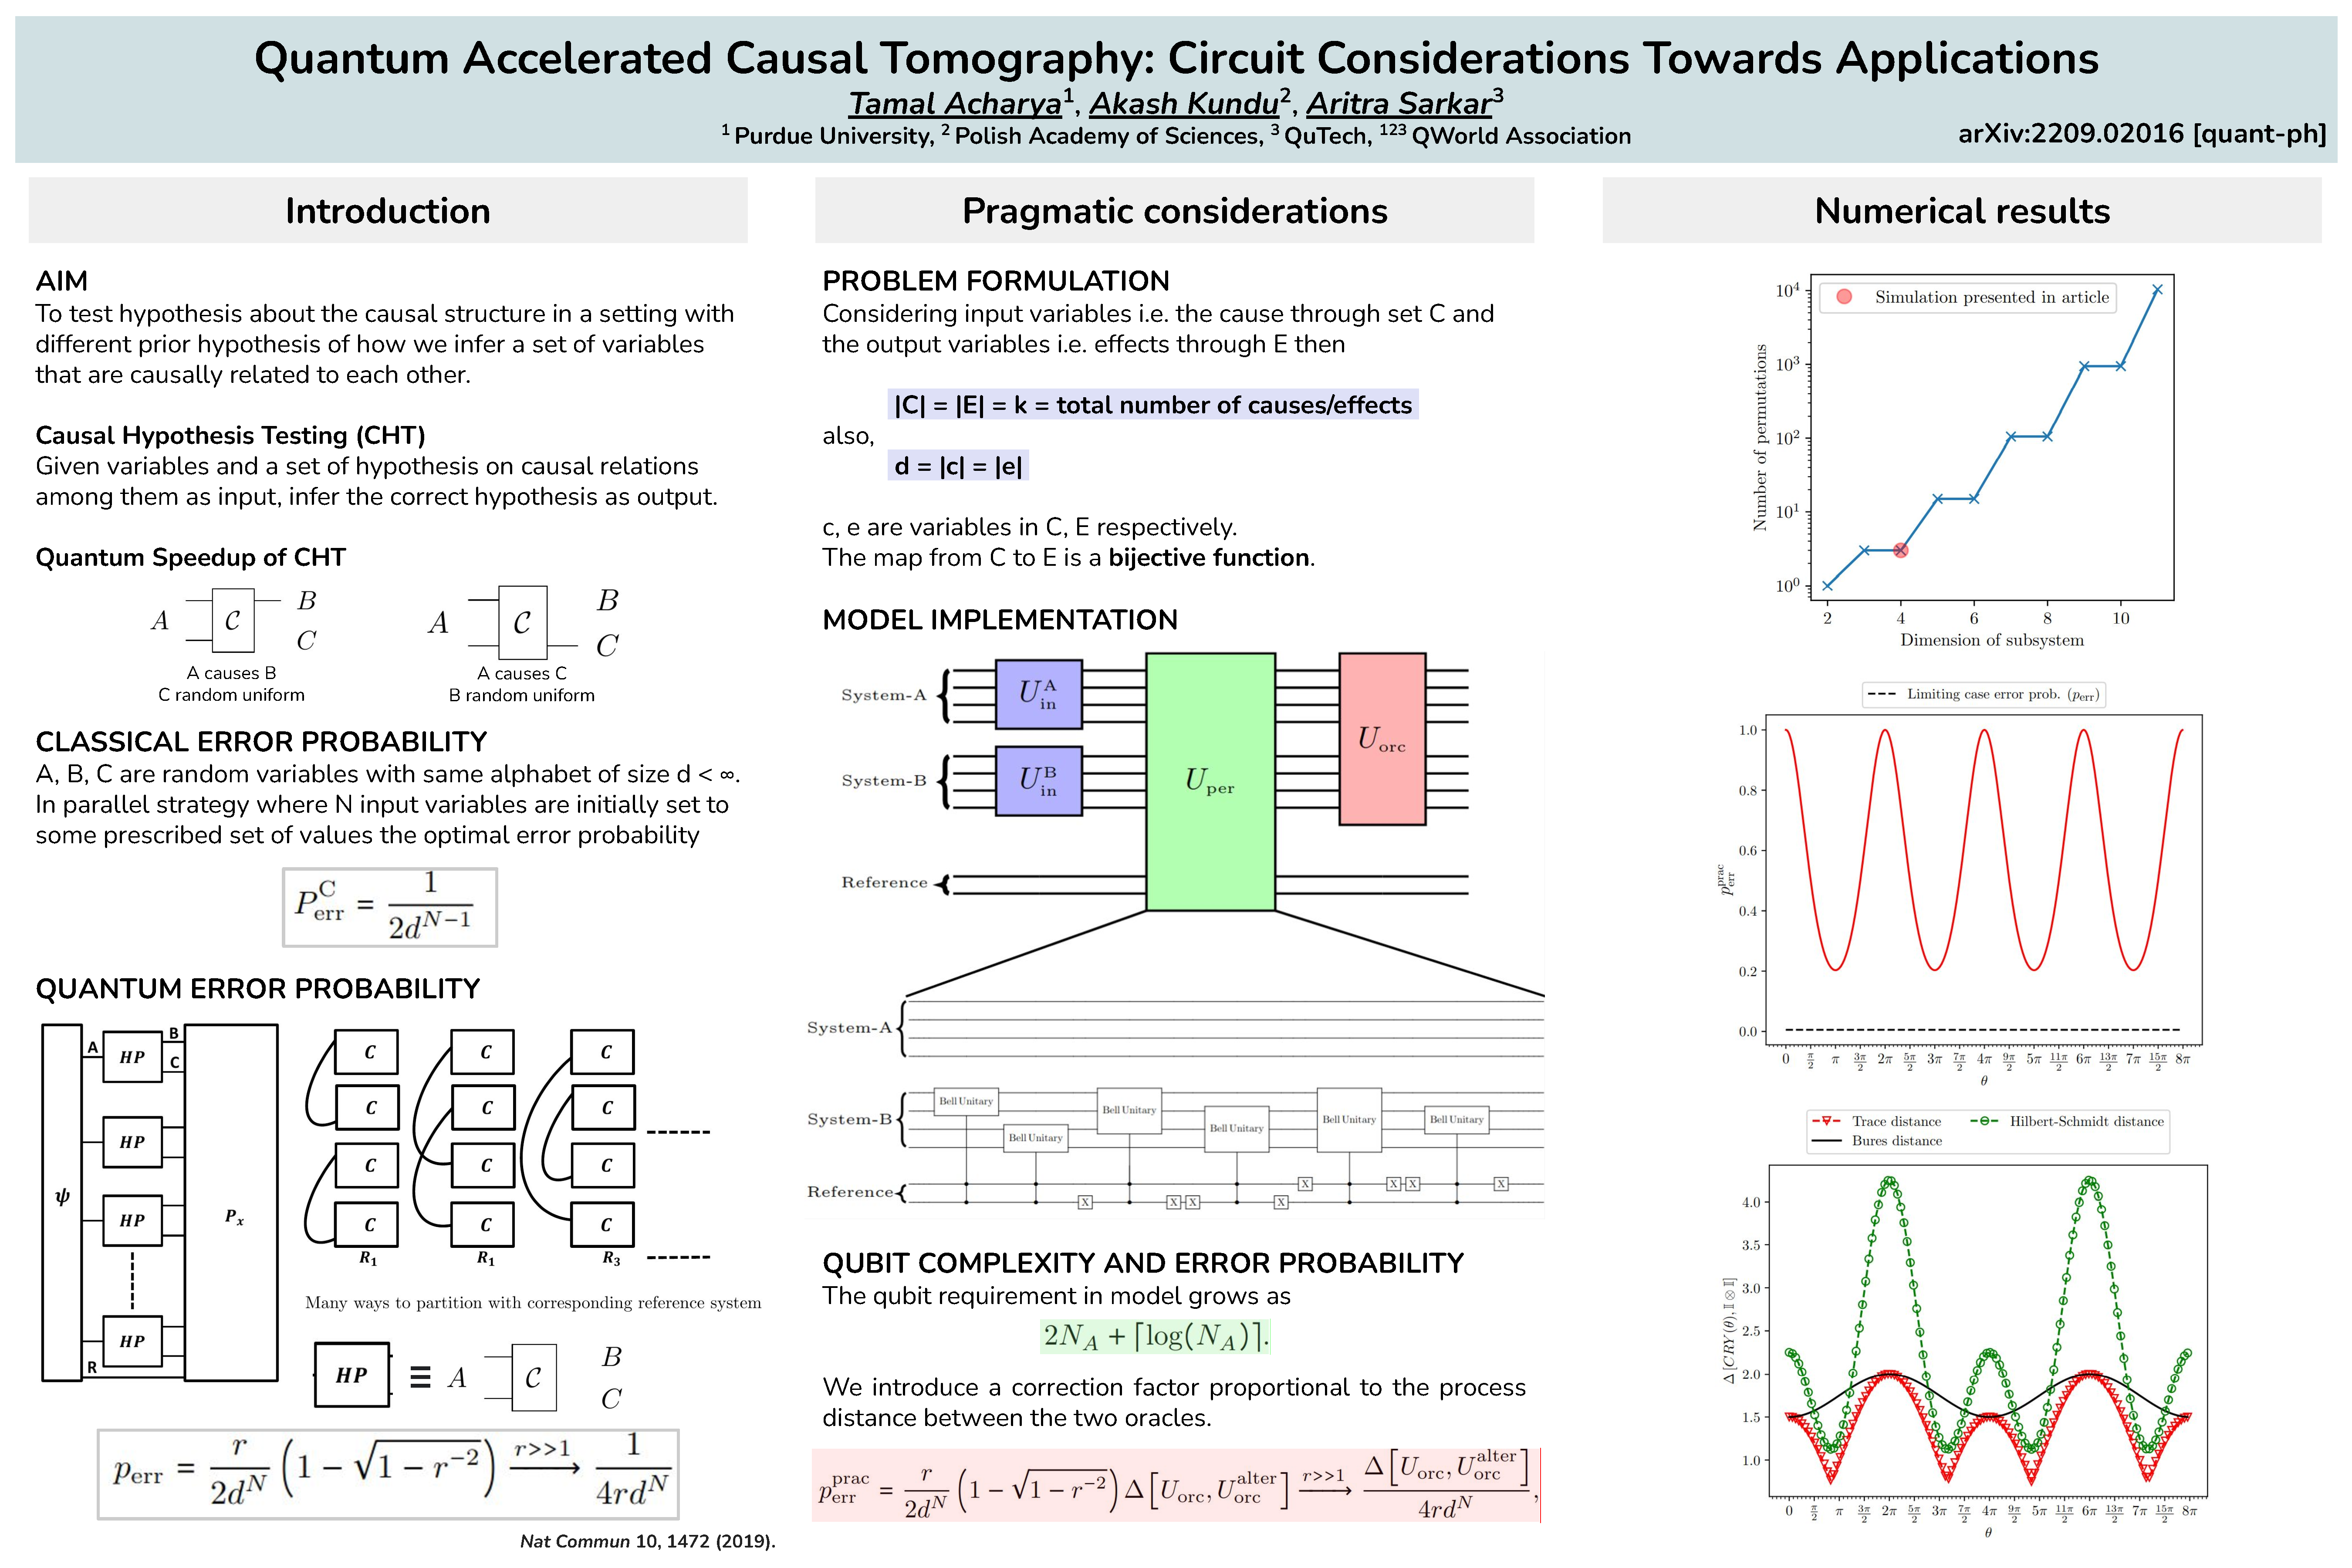
\includegraphics[width = \linewidth]{poster/practical_error_probability.pdf}
  %  \caption{The poster.}
  %  \label{fig:my_label}
%\end{figure*}

\nocite{*}
\bibliography{aipsamp}% Produces the bibliography via BibTeX.

\end{document}
%
% ****** End of file aipsamp.tex ******
